\documentclass[fleqn]{article}
\usepackage[utf8]{inputenc}
\usepackage[margin=2.5cm]{geometry}

% custom header/footer
\usepackage{fancyhdr}
\pagestyle{fancy}
\renewcommand{\headrulewidth}{0pt}
\fancyhf{}
\rfoot{\textsf{\thepage}}
\lfoot{\textsf{Suzie Brown}}

% tikz
\usepackage{tikz}
\usetikzlibrary{positioning}

%% maths
\usepackage{amsmath}
\usepackage{amssymb}
%\usepackage{amsthm}
%\newtheorem{corollary}{Corollary}
%\theoremstyle{definition}
%\newtheorem{defn}{Definition}
%
%% useful math symbols
\newcommand{\Prob}{\mathbb{P}}
\newcommand{\flnw}{\lfloor N w \rfloor}
%\newcommand{\E}{\mathbb{E}}
%\newcommand{\V}{\operatorname{Var}}
%\newcommand{\eqdist}{\overset{d}{=}}
%\newcommand{\I}[1]{\mathbb{I}\{#1\}}
%\newcommand{\Ntoinfty}{\overset{N\to\infty}{\longrightarrow}}
%\newcommand{\limNtoinfty}{\underset{N\to\infty}{\lim}}
%\newcommand\indep{\protect\mathpalette{\protect\independenT}{\perp}}
%\def\independenT#1#2{\mathrel{\rlap{$#1#2$}\mkern2mu{#1#2}}}
%
%% distributions
%\newcommand{\Cat}{\operatorname{Categorical}}
%\newcommand{\Unif}{\operatorname{Uniform}}
%\newcommand{\Mn}{\operatorname{Multinomial}}
%\newcommand{\Bin}{\operatorname{Binomial}}
%
%% project-specific commands
%\newcommand{\F}{\mathcal{F}_{t-1}}
%\newcommand{\vt}[2][t]{v_{#1}^{(#2)}}
%\newcommand{\wt}[2][t]{w_{#1}^{(#2)}}
%\newcommand{\wbar}[2][t]{\bar{w}_{#1}^{(#2)}}
%\newcommand{\vttilde}[2][t]{\tilde{v}_{#1}^{(#2)}}

\title{Stratified resampling: towards a finite time-scale}
\author{Suzie Brown}
\date{16th March 2021}

\begin{document}
\maketitle
\thispagestyle{fancy}

The aim of this note is to calculate (bounds on) the probabilities of the four different outcomes that are possible for the marginal offspring count $\nu_t^{(i)}$ conditional on $w_t^{(i)}$, under stratified resampling.
Ultimately, these bounds will be used to prove that the time-scale is finite
(i.e.\ $\Prob[\tau_N(t)=\infty]=0$ for all finite $t$)
under stratified resampling, assuming the additional constraints:
\begin{itemize}
\item that the weights are bounded away from the degenerate case $(1,\dots,1)/N$ in some way
\item that the transition densities $q_t(x,x^\prime)$ are uniformly bounded above and away from zero.
\end{itemize}
Once the probabilities are calculated (in the following), a proof similar to the one used to prove the finite time-scale condition for stochastic rounding will prove the same for stratified resampling.
The corresponding probabilities and hence finite time-scale proof for residual-stratified resampling should follow relatively easily by applying the bounds here within the residual resampling set-up.


\section*{Let's do it!}
Consider the marginal distribution of one offspring count $\nu_t^{(i)}$ conditional on the corresponding weight $w_t^{(i)}$. Henceforth we drop from the notation the dependence on $t$ and $i$, which are to be considered fixed throughout the following.
As we have already seen, the possible values of $\nu$ are restricted conditional on $w$ to $\{ \flnw-1, \flnw, \flnw+1, \flnw+2 \}$. Denote by $p_i$ the conditional probability $\Prob[ \nu = \flnw + i \mid w ]$, for $i = -1,0,1,2$.

We consider first a specific case (of particular interest for the finite time-scale proof) where $w= (1+\delta)/N$, with $\delta \in [0,1)$.
First let's look at $p_0 = \Prob[ \nu = 1 \mid w = (1+\delta)/N ]$.
Thinking about the inversion sampling schematic, %(Figure ??),
the resampling probabilities will depend upon where the length-$w$ interval falls with respect to the length-$(1/N)$ intervals for sampling. We split the possibilities into three cases (Figure~\ref{fig:cases}).

\begin{figure}[ht]
\centering
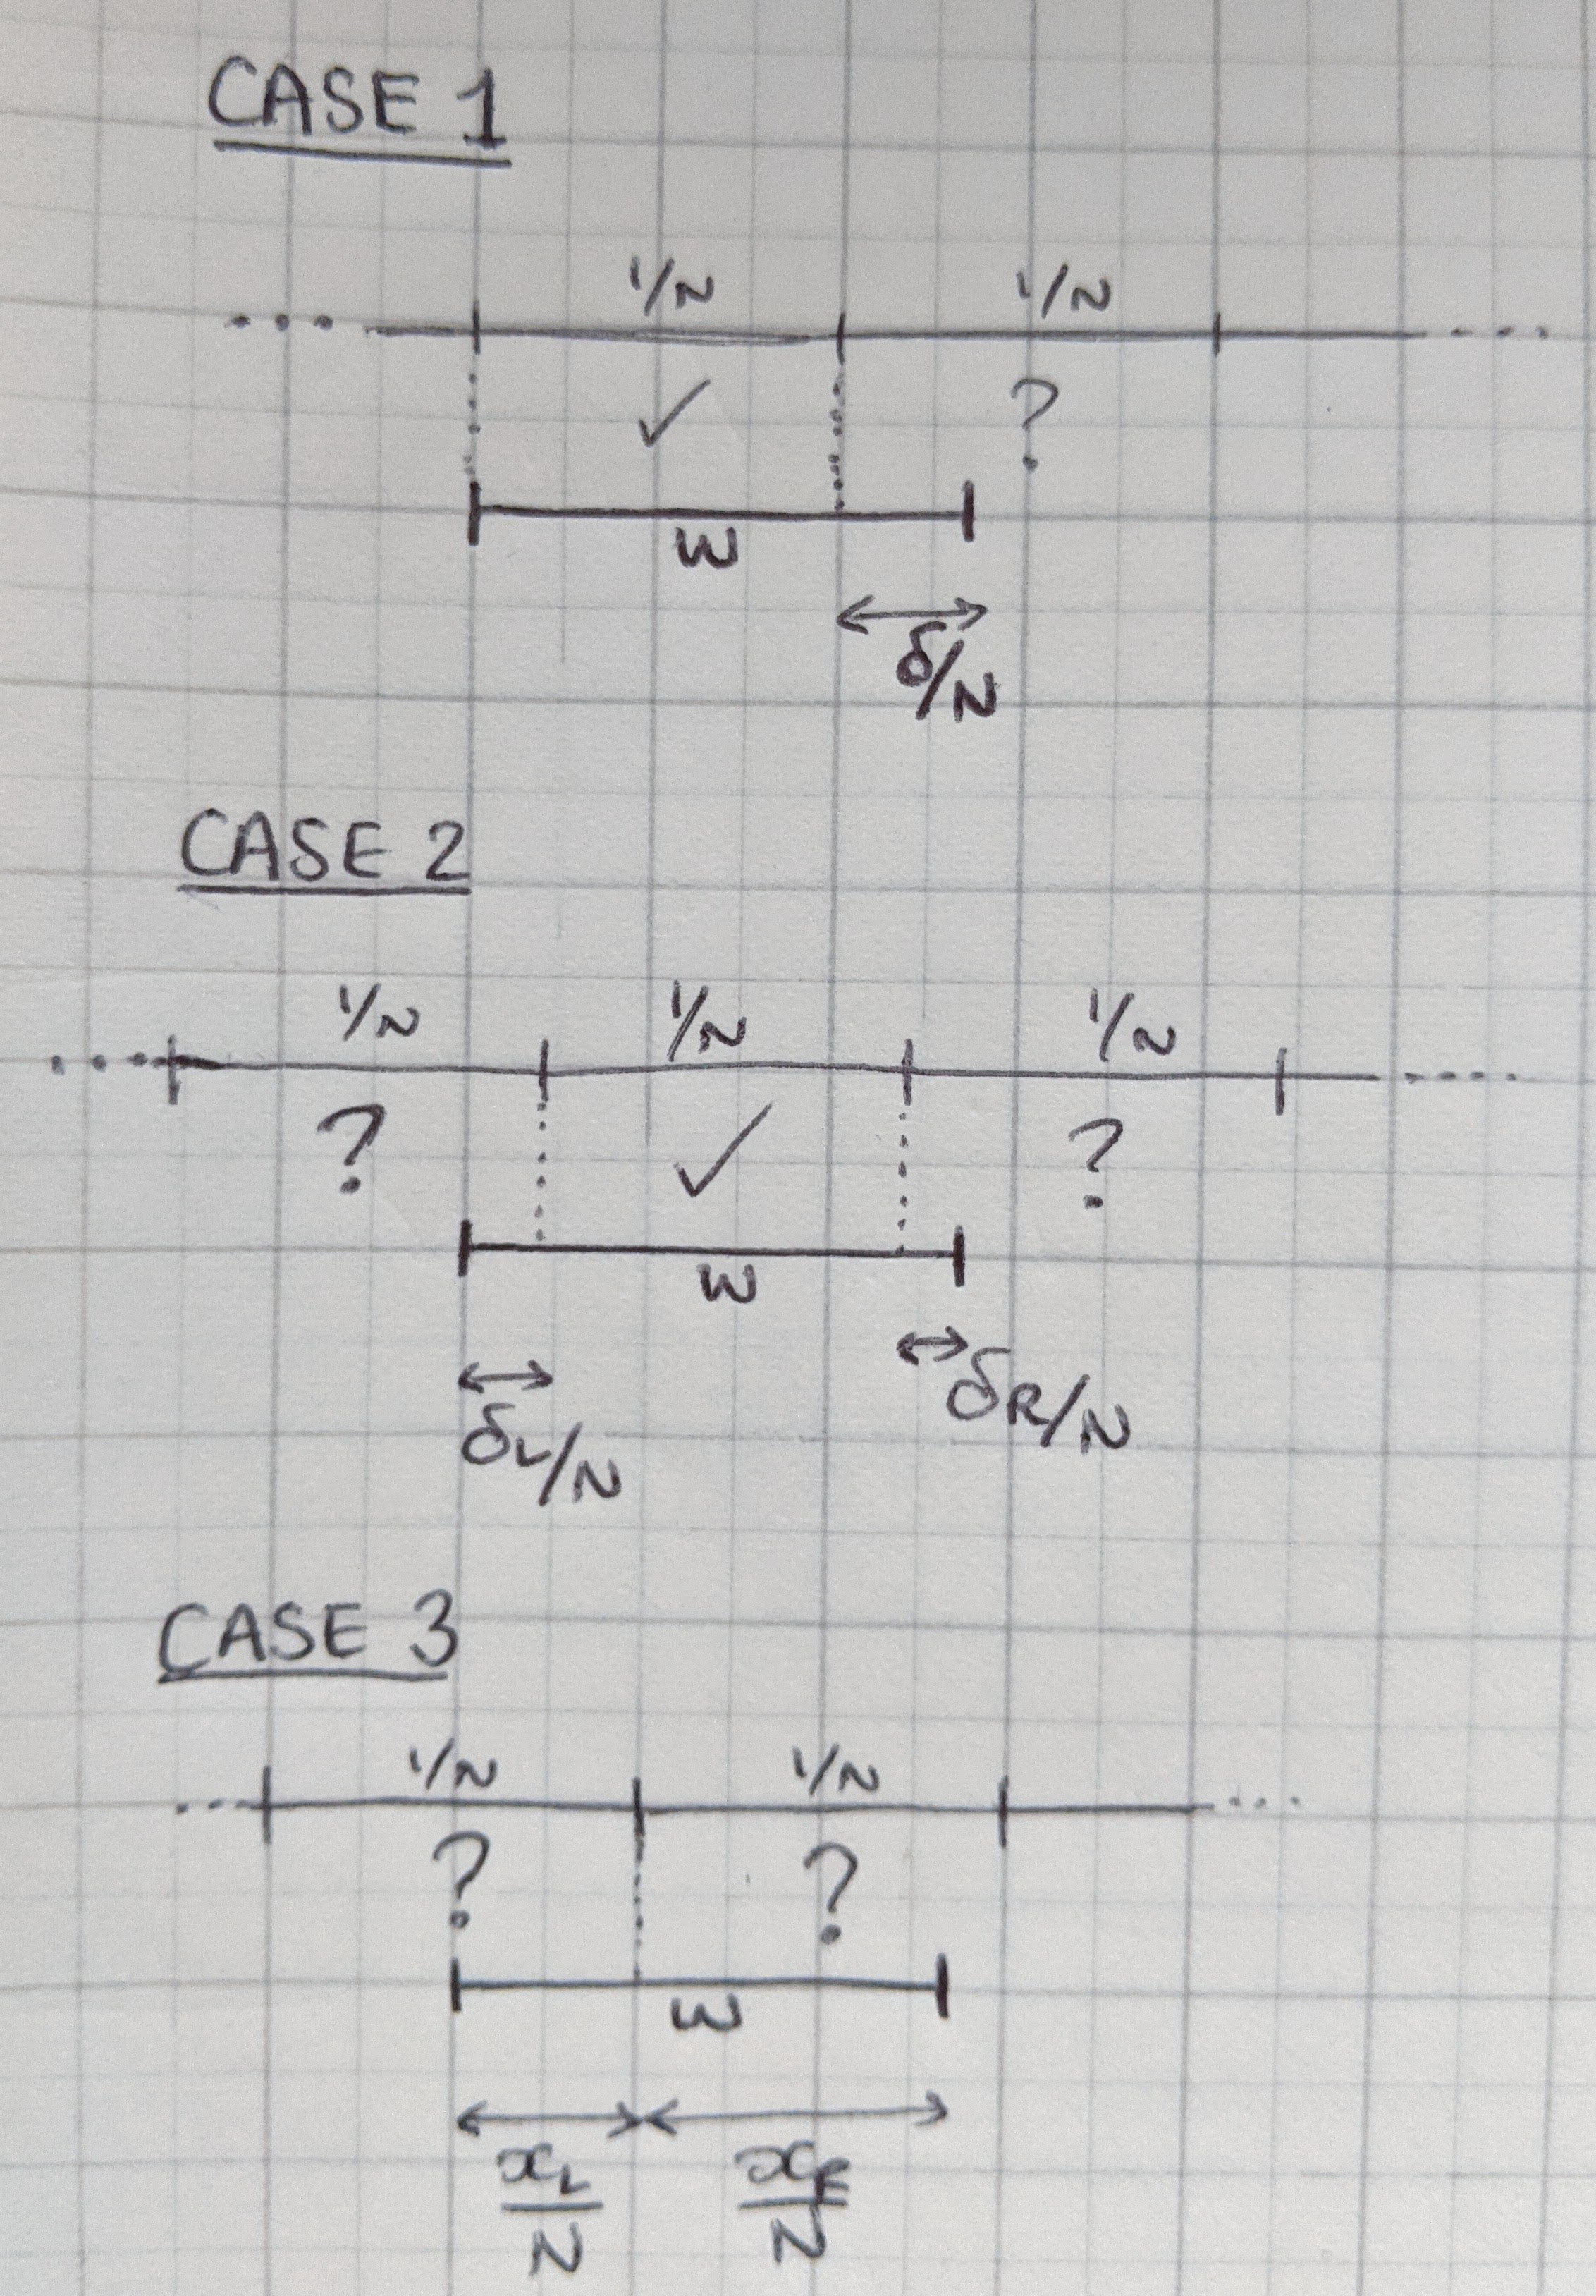
\includegraphics[width=0.5\textwidth]{cases_sketch.jpg}
\caption{Sketch illustrating the difference between Cases 1--3.}
\label{fig:cases}
\end{figure}

\subsection*{Case 1}
In this case, one offspring is assigned almost surely from the interval that is entirely overlapping. Thus $p_0$ is just the probability that the partially overlapping interval does not contribute a second offspring to $\nu$.
Hence,
\begin{equation}
p_0 
= \left( \frac{1}{N} - \frac{\delta}{N} \right) \div \frac{1}{N}
= 1-\delta .
\end{equation}

\subsection*{Case 2}
In this case, one offspring is assigned almost surely from the interval that is entirely overlapping. Thus $p_0$ is just the probability that neither of the partially overlapping intervals contributes a second offspring to $\nu$. 
The lengths are such that $\delta_L + \delta_R = \delta$.
We have
\begin{equation}
p_0 
= (1- \delta_L)(1- \delta_R)
= 1- \delta + \delta_L \delta_R .
\end{equation}
Noting that $\delta_L \delta_R \leq \delta^2/4 \leq \delta/4$, we conclude that
\begin{equation}
p_0 \in \left[ 1-\delta, 1- \frac{3\delta}{4} \right] .
\end{equation}
When $\delta_L \in \{0, \delta \}$, this case collapses to Case 1, which is consistent with the bounds derived here.

\subsection*{Case 3}
Here $p_0$ is the probability that exactly one of the partially overlapping intervals contributes an offspring to $\nu$. 
The lengths are such that $x_L + x_R = 1+\delta$, and also $x_L, x_R \in [\delta,1]$ (otherwise we would be in Case 2).
We have
\begin{equation}
p_0 
= x_L(1-x_R) + x_R(1-x_L)
= 1 + \delta - 2x_Lx_R .
\end{equation}
Notice that $\delta \leq x_Lx_R \leq (1+\delta)^2/4$, hence
\begin{equation}
p_0 \in \left[ \frac{1-\delta^2}{2}, 1-\delta \right] .
\end{equation}
When $\delta_L \in \{\delta, 1 \}$, this case collapses to Case 1, which is consistent with the bounds derived here.

\subsection*{Altogether}
Overall, then, we have the bounds
\begin{equation}
p_0 \in \left[ \frac{1-\delta}{2}, 1- \frac{3\delta}{4} \right] .
\end{equation}


\section*{Another thing}
Now let $w= 2+\delta$ for some $\delta \in [0,1)$.
Let's calculate $p_{-1} = \Prob[ \nu = 1 \mid w = (2+\delta)/N ]$.
Again thinking about how the inversion sampling intervals could fall, there is only one case in which $p_{-1}$ is non-zero (Figure \ref{fig:cases2}).
\begin{figure}[ht]
\centering
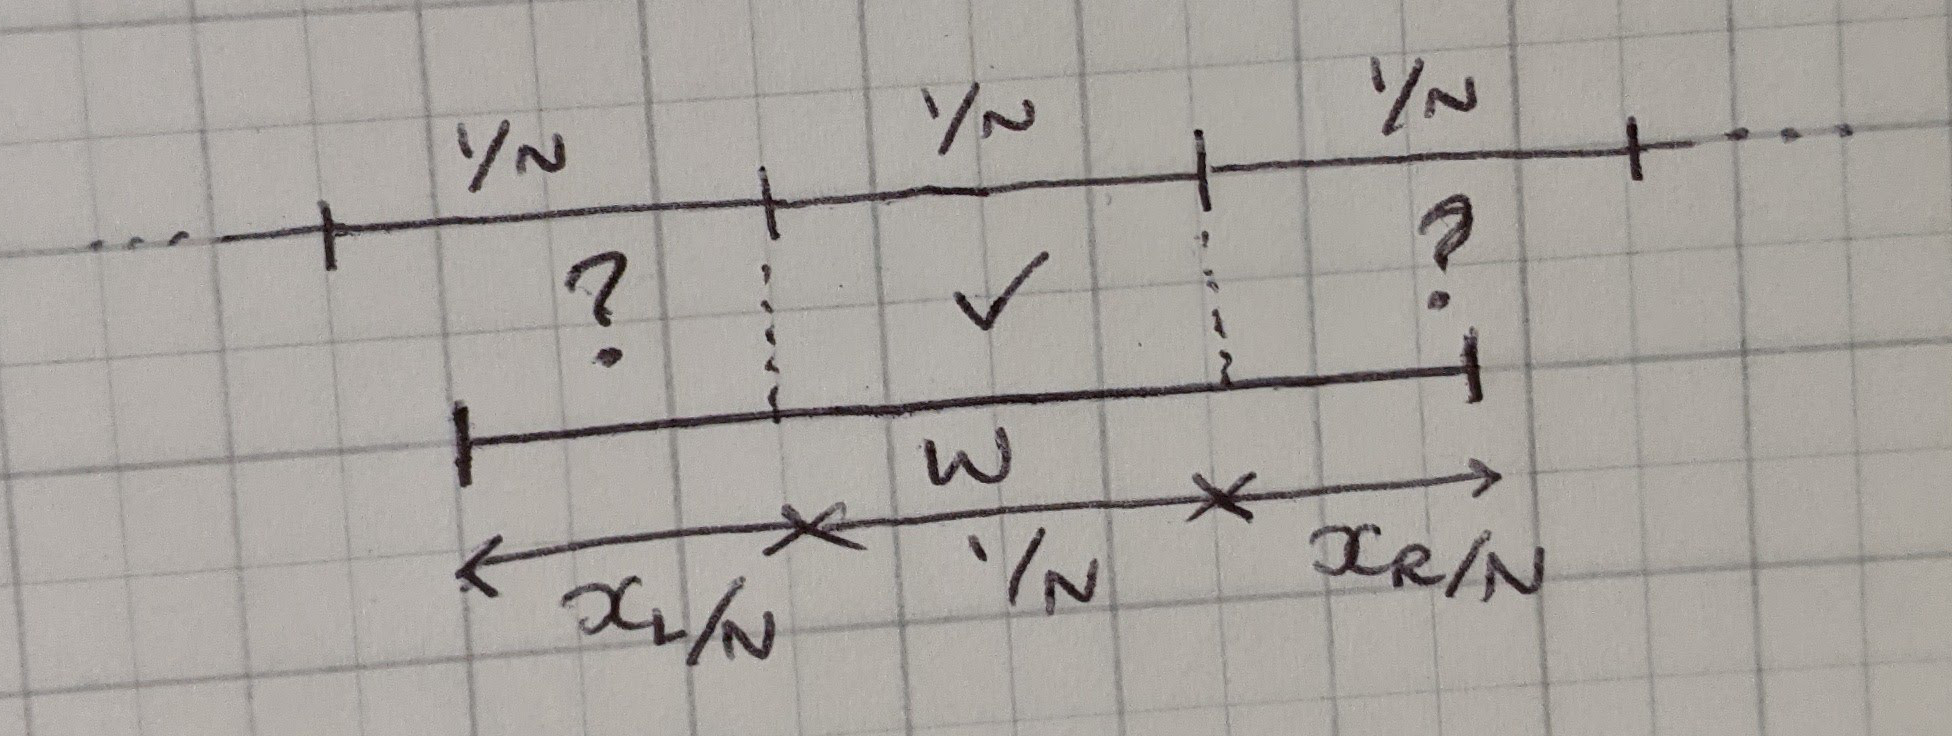
\includegraphics[width=0.5\textwidth]{cases2_sketch.jpg}
\caption{The only case giving non-zero probability $p_{-1}$.}
\label{fig:cases2}
\end{figure}
In this case,
\begin{equation}
p_{-1} 
= (1-x_L)(1-x_R)
= (1-x_L)(x_L - \delta) .
\end{equation}
This is a negative quadratic in $x_L$, with its unique maximum at $x_L=x_R= (1+\delta)/2$.
The maximum value of $p_{-1}$ is then
\begin{equation}
p_{-1}
= \frac{1}{4} (1 - \delta)^2
\leq \frac{1}{4}
\end{equation}
independently of $\delta$.
So we have, for any $\delta$,
\begin{equation}
p_{-1} \in \left[ 0, \frac{1}{4} \right] .
\end{equation}








\end{document}
